
\subsection{Udgangsfilter}
I 2. iteration blev der observeret store switching-spikes på udgangssignalet. Derfor blev det besluttet, at tilføre filtrering af disse spikes i 3. iteration. Den nødvendige kapacitet for udgangskondensatoren, blev realiseret ved fire kondensatorer i parallel. Kondensatorerne blev forbundet med ledninger på ca. $30mm$, som det ses på figur~\ref{fig:udgangsfilter}. Med en tommelfingerregel, der siger, man har selvinduktion på $1nH/mm$\cite{rule_of_thumb}, vil ledningerne og kondensatorerne derfor skabe fire LC-filtre i serie. Ved at placere udgangen efter disse filtre, blev der opnået en filtrering af spikes'ne uden yderligere tilføjelse af komponenter. 

\begin{figure}[H]
	\centering
	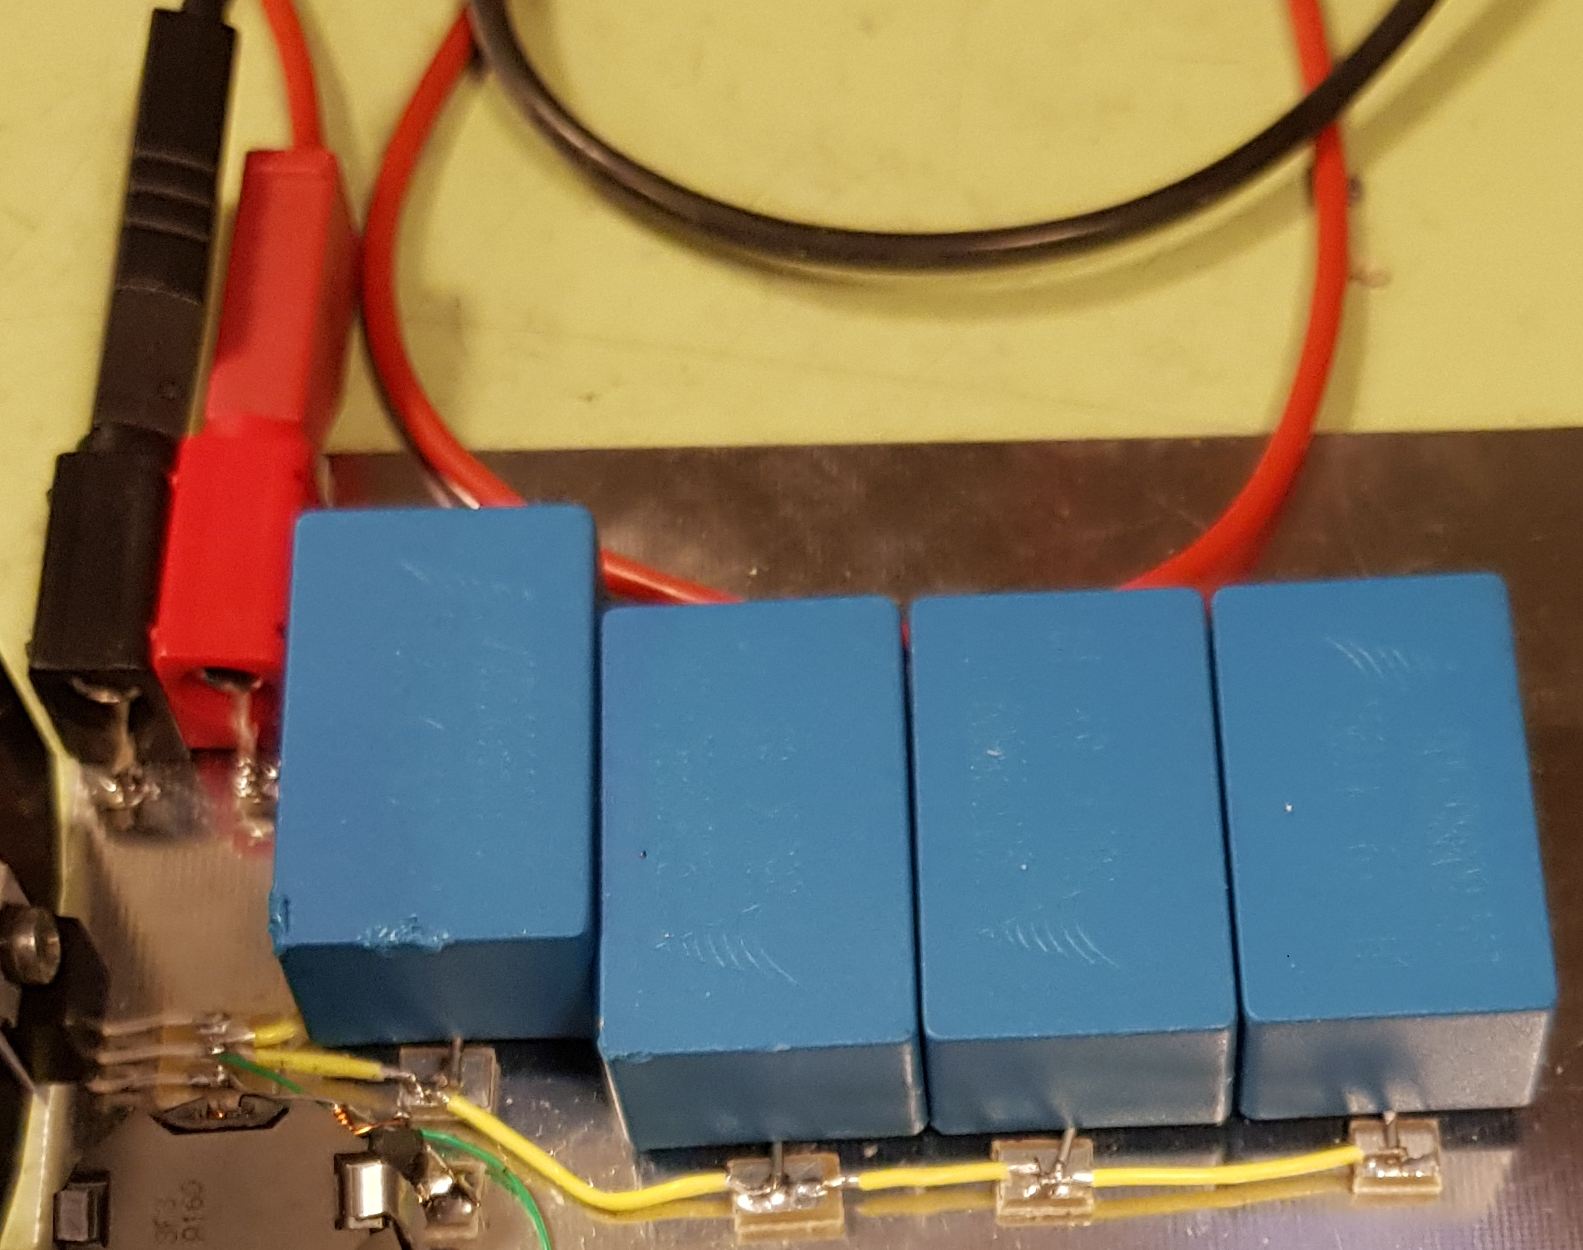
\includegraphics[width=0.5\linewidth]{../Dokumentation/tex/3iteration/Billeder/Analyse/Udgangsfilter_2iteration.png}
	\caption{Realisering af udgangsfilter efter 2. iteration}
	\label{fig:udgangsfilter}
\end{figure}

\noindent En nærmere analyse af udgangsfilteret er beskrevet i dokumentationens afsnit 6.4.